\documentclass{article}

\usepackage{polski}
\usepackage[utf8]{inputenc}
\usepackage[hidelinks]{hyperref}
\usepackage{caption}
\usepackage{graphicx}
\usepackage{float}
\usepackage{relsize}
\usepackage{chngcntr}
\counterwithin{figure}{section}

\newcommand{\insertprojectname}{\textit{Sesame }}
\title{
    Ochrona Danych
    \\
    [0.2em]\smaller{}
    Projekt
    \\
    Menadżer haseł \insertprojectname}
\author{
    Patryk Mroczyński 126810
    \\
    patryk.mroczynski@student.put.poznan.pl
    \\
    Daniel Staśczak 126816
    \\
    daniel.stasczak@student.put.poznan.pl
    \\
    Jakub Wiśniewski 126824
    \\
    jakub.t.wisniewski@student.put.poznan.pl
}
\date{\today}

\begin{document}
    \maketitle

    \newpage
    \tableofcontents
    \listoffigures

    \newpage

    \section{Charakterystyka ogólna projektu}
    \paragraph{}Aplikacja \insertprojectname jest menadżerem haseł, ułatwiającym zarządzanie unikalnymi i bezpiecznymi hasłami w różnych serwisach. Umożliwia ona bezpieczne przechowywanie haseł na serwerze oraz zezwala na dostęp do nich tylko dla użytkownika, który zna hasło do serwisu. Użytkownik ma możliwość wprowadzenia wpisu do bazy danych, który zawiera zaszyfrowane dane używane przy logowaniu do danego serwisu oraz etykietę, która ułatwia użytkownikowi zidentyfikowanie do jakiego celu przechowywane są dane we wpisie. Szyfrowanie oraz odszyfrowanie dzieje się po stronie klienta, dzięki czemu niemożliwa jest ingerencja osób mających dostęp do serwera. Operacje te są zautomatyzowane, dzięki czemu użytkownik nie musi posiadać wiedzy dotyczącej kryptografii.

    \section{Architektura systemu}
    \paragraph{}System oparty jest na modelu klient-serwer. Aplikacje klienckie udostępniają interfejs graficzny, umożliwiający korzystanie z serwisu osobom nietechnicznym. Na maszynie serwerowej uruchomiona jest relacyjna baza danych oraz program udostępniający API aplikacjom klienckim. API serwerowe pozwala wykonywać użytkownikom udostępnione operacje na bazie danych. W oparciu o API serwerowe, stworzone zostały API klienckie w poszczególnych językach programowaniach, które są dedykowane konkretnym platformom i które udostępniają funkcjonalności ułatwiające implementacje aplikacji klienckich.

    \subsection{Baza danych}
    \paragraph{}Baza danych, przedstawiona na rysunku \ref{fig:db} zawiera informacje o tabelach wykorzystywanych w serwisie. Tabele user, password oraz device stanowią bazę dla głównej funkcjonalności w serwisie, a wszystkie pozostałe tabele są tabelami pomocniczymi --- udostępniają dodatkowe funkcjonalności, zwiększające atrakcyjność serwisu i bezpieczeństwo przetrzymywanych informacji wrażliwych. Tabela user zawiera informacje o użytkowniku, niezbędne do prawidłowego i bezpiecznego funkcjonowania aplikacji oraz umożliwiające użytkownikom korzystanie z funkcjonalności systemu. Tabela password zawiera wpisy zawierające zaszyfrowane hasła dla konkretnych użytkowników, a tabela device umożliwia korzystanie z aplikacji tylko zweryfikowanym przez użytkownika urządzeniom. Tabela encrypting\_algorithm umożliwia zdefiniowanie nowych metod szyfrowania haseł, nie tracąc jednocześnie informacji o metodach stosowanych przy szyfrowaniu poprzednich haseł. Informacja o wykorzystanym algorytmie znajduje się w tabeli password jako klucz obcy. Tabela device\_type umożliwia przechowywanie informacji o typie urządzenia. Nie jest ona obecnie wykorzystywana, ale zbierane przez nią informacje mogą posłużyć do rozbudowania serwisu o dodatkowe funkcjonalności takie jak autoryzacja dwuetapowa.

    \begin{figure}[H]
		\centering
		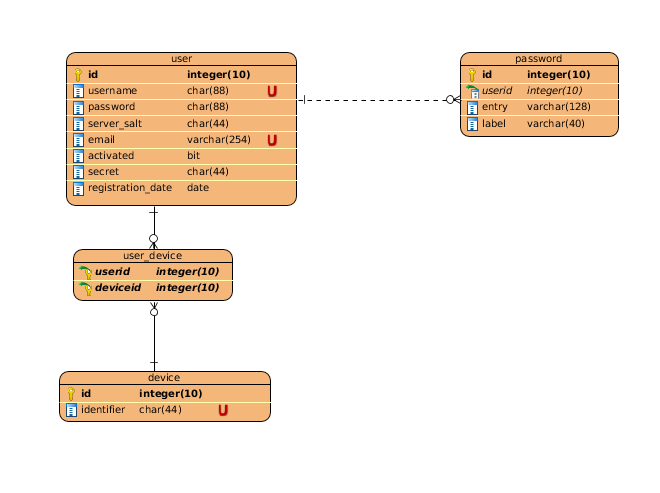
\includegraphics[width=1\linewidth]{assets/db.png}
		\caption{Model bazy danych}
		\label{fig:db}
	\end{figure}

    \subsection{Serwisy}
    \paragraph{} Aplikacja serwerowa udostępnia szereg serwisów, które są wykorzystywane do komunikacji pomiędzy klientem i serwerem. Serwisy stanowiące trzon funkcjonalności systemu to:
    \begin{itemize}
        \item AuthService --- System umożliwiający użytkownikom utworzenia konta w serwisie, służący do aktywacji konta oraz udostępniający możliwość wygenerowania tokenów JWT, używanych do dalszej autoryzacji w serwisie.
        \item UserService --- Pozwala na pobranie informacji o użytkowniku takich jak adres email, data rejestracji itp. Umożliwia zmianę poszczególnych danych użytkownika (np. głównego hasła). Do wykonywania operacji na tym serwisie wymagany jest token uwierzytelniający JWT.
        \item PasswordService --- Udostępnia metody pozwalające na zarządzanie przetrzymywanymi hasłami w serwisie. Pozwala pobrać listę etykiet haseł, dodać nowe hasło, usunąć hasło oraz pobrać hasło na podstawie etykiety. Serwis ten wymaga użycia tokenu JWT w celach autoryzacyjnych.
    \end{itemize}

    \section{Bezpieczeństwo}
    \paragraph{}W rozdziale opisane zostały wszystkie zastosowane w aplikacji aspekty bezpieczeństwa. Wymienione zostały wszystkie zastosowane mechanizmy na każdym etapie działania systemu.

    \paragraph{}Mechanizmem zabezpieczającym ujawnienie hasła użytkownika poprzez wyciek informacji z bazy danych jest wykorzystanie funkcji PBKDF2, która zapewnia większe bezpieczeństwo od używania funkcji skrótu. Została ona zaprojektowana do utrudnienia prób ataków brute-force oraz słownikowych. Wydłuża ona czas potrzebny na obliczenie pojedynczego skrótu w stopniu zależnym od zastosowanej liczby iteracji, a wykorzystanie soli, która jest indywidualna dla każdego użytkownika i dodawana do każdego hasła, zapewnia różne skróty dla identycznych haseł różnych użytkowników. Dzięki temu zmniejszona jest skuteczność tablic tęczowych --- atakujący musiałby tworzyć osobne tablice dla każdej soli.

    \paragraph{}Dzięki użyciu protokołu HTTPS, przechwycenie przesyłanych danych jest bardzo trudne, ale pozostaje problem widoczności nieprzetworzonego hasła po stronie serwera. Aby zabezpieczyć użytkowników przed wykorzystaniem tego faktu przez atakujących, wykorzystana zostaje ponownie funkcja PBKDF2, tym razem po stronie klienta. Jako sól użyty zostaje wynik funkcji skrótu nieprzetworzonej nazwy użytkownika w połączeniu z nieprzetworzonym hasłem, a liczba iteracji jest mniejsza niż po stronie serwerowej, aby użytkownik nie odczuł wykonywanych operacji. Sama nazwa użytkownika zostaje przesłana na serwer jako wynik funkcji skrótu.

    \paragraph{}Aby zmniejszyć prawdopodobieństwo przechwycenia pakietu zawierającego hasło użytkownika, wykorzystane zostały tokeny JWT. Dzięki temu aplikacja kliencka po poprawnym logowaniu otrzymuje token zawierający informacje niezbędne do wykonywania kolejnych zapytań (takie jak skrót nazwy użytkownika czy czas wygaśnięcia tokenu). Całość tokenu jest podpisana za pomocą algorytmu kryptograficznego HMAC, wykorzystującego sekret serwerowy, co zapewnia autentyczność i nienaruszalność tych danych. Dodatkowo dodawany jest kolejny sekret (przechowywany w bazie danych), który jest unikalny dla każdego użytkownika, dzięki czemu, po jego wykryciu sekretu serwerowego przez atakującego, niemożliwe jest fałszowanie podpisu dla każdego użytkownika. Sekret serwerowy jest zmieniany co określony odcinek czasu.

    \paragraph{}Każdorazowe logowanie na nowym (nieautoryzowanym wcześniej) urządzeniu powoduje wysłanie wiadomości e-mail do użytkownika, aby ten mógł zweryfikować czy akcja została wykonana na jego urządzeniu, czy jest to próba włamania. Dzięki zastosowaniu tego mechanizmu, dostęp do danych użytkownika otrzymują tylko urządzenia należące do niego. Aby umożliwić takie zabezpieczenie, aplikacja kliencka musi wysyłać skrót swojego identyfikatora, którym może być np. adres MAC komputera czy fingerprint przeglądarki. Dopiero po poprawnym zweryfikowaniu hasła i identyfikatora, generowany jest token JWT, którego czas wygaśnięcia to krótki odcinek czasu (dzięki czemu nawet w przypadku przechwycenia tokenu, atakujący można korzystać z niego tylko przez chwilę).

    \paragraph{}Po każdej interakcji aplikacji klienckiej z serwerem, zostaje dodany wpis do logów, który zawiera informacje o użytkowniku, adresie IP, akcji, która została wykonana oraz o powodzeniu akcji. Dzięki temu zapewniona jest niezaprzeczalność i rozliczalność, co pozwala na śledzenie podejrzanych aktywności oraz przeciwdziałanie im.

    \paragraph{}Hasła zapisane przez użytkownika, przechowywane na serwerze są w postaci zaszyfrowanej symetrycznie. Użytkownik może wybrać czy do odszyfrowania hasła chce używać zmodyfikowanego przez aplikację kliencką hasła do serwisu czy użyć osobnego klucza, podanego przez użytkownika. Całość szyfrowania i deszyfrowania odbywa się w aplikacji klienckiej, dzięki czemu klucz nigdy nie wydostaje się poza urządzenie użytkownika.

    \paragraph{}Do generowania soli oraz sekretów po stronie serwera używane są algorytmy wykorzystujące kryptograficznie bezpieczne źródło losowości (np. \texttt{/dev/urandom} w przypadku systemów opartych o UNIX lub \texttt{CryptGenRandom} w przypadku systemów Windows).


    %jwt - DONE, hashe - DONE, https - DONE, zautoryzowane urządzenia - DONE, logi - DONE, enkrypcja haseł - DONE, generowane tokeny(z sekretem), /dev/urandom



    \section{Wymagania}
    \paragraph{}W rozdziale zostały opisane wymagania funkcjonalne oraz niefunkcjonalne serwera, aplikacji klienckich oraz komunikacji między nimi wraz z podziałem na aktorów.

    \subsection{Wymagania funkcjonalne}
    W tej sekcji przedstawione zostały wymagania funkcjonalne z podziałem na dwóch aktorów --- użytkownika niezalogowanego i użytkownika zalogowanego.

    \begin{itemize}
		\item Niezalogowany użytkownik
			\begin{itemize}
				\item Możliwość utworzenia konta w serwisie.
				\item Możliwość zalogowania do serwisu za pomocą hasła głównego i nazwy użytkownika.
			\end{itemize}

		\item Zalogowany użytkownik
			\begin{itemize}
				\item Możliwość wylogowania.
				\item Możliwość edycji w opcjach konta adresu email oraz hasła głównego.
				\item Możliwość dodania nowego przechowywanego hasła do serwisu wraz z informacjami dodatkowymi --- etykietą i nazwą użytkownika.
				\item Możliwość usunięcia hasła przechowywanego.
				\item Możliwość edycji hasła przechowywanego oraz informacji dodatkowych.
				\item Możliwość wyświetlenia etykiet przechowywanych haseł.
				\item Możliwość wyboru etykiety i przekopiowania do schowka hasła lub nazwy użytkownika dla danego wpisu.
			\end{itemize}
	\end{itemize}

    \subsection{Wymagania niefunkcjonalne}
    W wymaganiach niefunkcjonalnych opisane są technologie jak i techniki związane z budową aplikacji klienckiej oraz serwerowej.
	\begin{itemize}
		\item Aplikacja serwerowa napisana w języku Python3.
		\item Aplikacja serwerowa umożliwiająca administratorowi wybór systemu relacyjnej bazy danych pomiędzy PostgreSQL, MySQL oraz SQLite3.
		\item Aplikacja serwerowa udostępnia publiczne API, na podstawie którego budowane mogą być aplikacje klienckie.
		\item Aby użytkownik mógł korzystać z aplikacji musi się poprawnie zalogować na założone w serwisie konto.
		\item Dane użytkownika są przechowywane w bazie danych.
		\item Główne hasło użytkownika przechowywane jest jako wynik funkcji rozciągania klucza PBKDF2 z wykorzystaniem algorytmu SHA512 i 100000 iteracji.
		\item Wszelkie wykorzystywane źródła losowe po stronie serwerowej powinny być kryptograficznie bezpieczne.
		\item Hasło użytkownika powinno posiadać minimum 16 znaków długości.
		\item System autoryzacji oparty jest o tokeny JWT.
		\item Aplikacje klienckie powinny udostępniać wszystkie najważniejsze funkcjonalności systemu.
		\item API stworzone jest zgodnie z architekturą REST, w formie serwisów.
		\item Hasła przechowywane w serwisie są szyfrowane za pomocą wybranej metody szyfrowania symetrycznego.
		\item Szyfrowanie i deszyfracja haseł odbywa się wyłącznie po stronie aplikacji klienckiej.
	\end{itemize}
    % Kryptograficznie bezpieczne źródło losowości dla aplikacji serwerowej.

    \section{Narzędzia, środowiska, biblioteki}
    \paragraph{}Serwer działa w oparciu o system operacyjny Ubuntu Server 18.04 LTS.
	Do zarządzania danymi wykorzystywana jest relacyjna baza danych PostgreSQL 10
	Mikroserwisy działające jako aplikacja serwerowa napisane są w języku Python 3.7 wraz z frameworkiem webowym CherryPy oraz biblioteką udostępniającą funkcjonalności ORM i łączności z bazą danych Peewee.
	\paragraph*{} Pierwsza aplikacja kliencka to aplikacja desktopowa napisana w języku Python 3.7, testowana na systemach operacyjnych Windows 10 oraz wybranych dystrybucjach Linuxa: Ubuntu 18.04 LTS i Antergos Linux. Biblioteką wykorzystaną w projekcie, która udostępnia funkcje ułatwiające tworzenie interfejsów użytkownika jest Tkinter.
	\paragraph*{} Dodatkowe narzędzia wykorzystane przy tworzeniu aplikacji to Visual Studio Code, Vim, DBeaver Community Edition 5 oraz Postman.
	\paragraph*{} Narzędzia, które zostały wykorzystane do wspierania pracy zespołowej to Discord do komunikacji głosowej podczas pracy, system kontroli wersji Git wraz z repozytorium na stronie GitHub.com, TeX Live do tworzenia dokumentacji oraz Visual Paradigm do tworzenia schematów oraz diagramów.

    \section{Możliwości rozwoju}
    W ty rozdziale omówione zostały możliwe kierunki rozwoju aplikacji.

    \begin{itemize}
		\item Wprowadzenie opcjonalnej autoryzacji dwuetapowej, umożliwiającej użytkownikom zwiększenie bezpieczeństwa przechowywanych w serwisie haseł. System ten mógłby zostać zaimplementowany w formie aplikacji mobilnej dostępnej w systemach Android i iOS, które po ówczesnym zalogowaniu i oznaczeniu urządzenia jako zaufanego mogłyby generować kilkucyfrowe kody autoryzacyjne.
		\item Udostępnienie większej ilości oficjalnych aplikacji klienckich, które mogłyby być dostępne jako aplikacje mobilne na systemy Android i iOS, rozszerzenie w przeglądarkach czy aplikacja przeglądarkowa.
		\item Ustalenie jednolitej szaty graficznej aplikacji klienckich i elementów ułatwiających rozpoznanie systemu takich jak logo czy kolorystyka.
        \item Wprowadzenie do Client API funkcjonalności sparametryzowanego generowania silnych haseł. Użytkownik końcowy mógłby ustalić m.in. pożądaną długość hasła i pulę znaków użytych w trakcie generowania (spośród małych i dużych liter, cyfr i znaków specjalnych).
        \item Wprowadzenie do Client API funkcjonalności analizy siły już zapisanych haseł.
	\end{itemize}

\end{document}
